\documentclass[conference,10pt,letterpaper]{IEEEtran}

\usepackage[utf8]{inputenc}
\usepackage[T1]{fontenc}
\usepackage{cite}
\usepackage{amsmath,amssymb}
\usepackage{array,booktabs,tabularx}
\usepackage{graphicx}
\usepackage{microtype}
\usepackage{xurl}
\usepackage[hidelinks]{hyperref}

\urlstyle{same}
\newcolumntype{Y}{>{\raggedright\arraybackslash}X}
\hyphenation{Web-Authn post-quantum crypto-graphic crypto-graphy micro-con-trol-ler}

\title{A New IoT Platform Based on PQC Algorithms: A Solution for Quantum Computing Threats}

\author{%
\IEEEauthorblockN{Nhat Phat Huynh, Dong Quan Nguyen, Quan Le, Thanh Hung Le, and Minh Son Nguyen\textsuperscript{1,2}}
\IEEEauthorblockA{\textsuperscript{1}University of Information Technology\\
\textsuperscript{2}Vietnam National University at HCM City\\
Ho Chi Minh City, Vietnam\\
\{24521294, 24521438, 24521429\}@gm.uit.edu.vn; hunglt@ms.uit.edu.vn; sonnm@uit.edu.vn}}

\hypersetup{
  pdftitle={A New IoT Platform Based on PQC Algorithms: A Solution for Quantum Computing Threats},
  pdfauthor={Nhat Phat Huynh; Dong Quan Nguyen; Quan Le; Thanh Hung Le; Minh Son Nguyen},
  pdfsubject={ACOMPA 2026 Paper \#4},
  pdfkeywords={post-quantum cryptography, Internet of Things, passkey, WebAuthn, ML-KEM, ML-DSA, SLH-DSA, RISC-V}
}

\begin{document}
\maketitle
\nocite{shor1997,banerjee2019,ye2024,carril2024,mao2023,karl2025,roma2021,liu2018,schoeffel2021,kannwischer2022,stebila2017,fips203,fips204,fips205,webauthn2026,rfc9964,nistir8547,goertzen2023}

\begin{abstract}
The migration from classical public-key cryptography to post-quantum cryptography is becoming important for Internet of Things (IoT) authentication, because large-scale quantum computers would undermine the RSA, Diffie-Hellman, and elliptic-curve assumptions used by many current authentication and key-establishment mechanisms. This paper proposes a scalable Edge-IoT post-quantum cryptography (PQC) platform that treats PQC deployment as a tiered system problem rather than a direct primitive replacement. The architecture assigns ML-KEM to session-key establishment, ML-DSA to challenge-response authentication at the node or gateway tier, and SLH-DSA to high-assurance but infrequent firmware, audit, and attestation tasks. To connect these algorithms to IoT workflows, the platform defines a PQC-aware passkey metadata object, a gateway-mediated hybrid migration policy, and an embedded data path that uses shared buffers and high-throughput peripheral paths. A software-centric evaluation on QEMU-based ARM64 and RISC-V targets, together with a concurrent stress workload, compares latency, memory, and payload size. The results indicate that ML-KEM and ML-DSA are practical building blocks for the measured node/gateway workflow, whereas SLH-DSA should be used selectively because of its large signatures and high signing latency.
\end{abstract}

\begin{IEEEkeywords}
Post-quantum cryptography, Internet of Things, passkey, WebAuthn, ML-KEM, ML-DSA, SLH-DSA, RISC-V
\end{IEEEkeywords}

\section{Introduction}

Quantum computing creates a long-term migration risk for IoT authentication. RSA, Diffie-Hellman, and elliptic-curve mechanisms rely on integer factorization or discrete-logarithm assumptions that are vulnerable to Shor's algorithm~\cite{shor1997}. This affects not only traditional key exchange and certificate-based authentication, but also passwordless systems whose credentials are still implemented with classical public-key signatures. IoT devices make the migration harder because they often operate with limited SRAM, flash, radio bandwidth, and energy budget. As a result, replacing a compact ECDSA or ECDH operation with a larger PQC object can change packet sizes, buffer allocation, credential storage, and end-to-end latency.

Prior work shows that PQC deployment cannot be treated as a direct drop-in replacement for classical public-key primitives. Configurable lattice crypto-processors and IoT-oriented PQC processors demonstrate that polynomial arithmetic, sampling, and memory organization dominate the cost of lattice-based cryptography~\cite{banerjee2019,ye2024}. FPGA and software-hardware co-design studies further show that Kyber/ML-KEM and Dilithium/ML-DSA benefit from dedicated acceleration and careful data movement~\cite{carril2024,mao2023}, while hash-oriented accelerators are relevant for SPHINCS+/SLH-DSA-style signatures~\cite{karl2025}. At the system level, energy, bandwidth, and communication cost must be evaluated together rather than as isolated runtime values~\cite{roma2021,liu2018,schoeffel2021}. This paper addresses the resulting migration gap through three contributions: a layered node/gateway/server architecture for PQC-enabled IoT, a PQC-aware passkey metadata and hybrid-policy model, and a measurement-driven placement rule that maps ML-KEM, ML-DSA, and SLH-DSA to the tiers where they are most practical.

The remainder of this paper is organized as follows. Section~II reviews NIST-standardized PQC algorithms, software ecosystems, WebAuthn/passkey migration, embedded communication constraints, and the migration gap in current IoT stacks. Section~III presents the proposed scalable Edge-IoT PQC architecture, including the tiered algorithm-placement model, PQC passkey object, hardware data path, enrollment and authentication flow, key rotation, and failure handling. Section~IV describes the QEMU-based ARM64/RISC-V evaluation and stress-test results, then discusses the design implications for buffering, gateway offloading, and hardware acceleration. Section~V concludes the paper and outlines future work on physical-board measurements and accelerator integration.

\section{Related Work}

\subsection{NIST PQC standards and software ecosystems}

ML-KEM, formerly CRYSTALS-Kyber, is a key-encapsulation mechanism based on module learning with errors. It provides a shared secret and ciphertext, but it is not intended to encrypt application data directly. A practical protocol uses ML-KEM to establish a session secret and then applies an authenticated-encryption scheme such as AES-GCM or ChaCha20-Poly1305 to the actual IoT payload. ML-DSA, formerly CRYSTALS-Dilithium, provides module-lattice-based digital signatures and is a candidate for recurring authentication when bandwidth and buffering are provisioned. SLH-DSA, derived from SPHINCS+, is hash-based and conservative, but its signatures are much larger and its signing procedure is slower than lattice-based alternatives~\cite{fips203,fips204,fips205}.

Open-source libraries also influence deployability. PQClean focuses on clean, portable, tested C implementations of post-quantum algorithms~\cite{kannwischer2022}, whereas the Open Quantum Safe project provides a higher-level software ecosystem for prototyping quantum-safe cryptography and integrating algorithms into Internet protocols~\cite{stebila2017}. These ecosystems are useful as reproducible software baselines before algorithm-specific hardware acceleration or board-level optimization is introduced.

\subsection{WebAuthn, passkeys, and quantum migration}

WebAuthn defines an API for creating and using scoped, attested, public-key credentials. A credential is created for a WebAuthn relying party, stored by an authenticator, and later used only for origins that belong to the same relying party. Authentication follows a challenge-response model in which the authenticator proves possession of the private key by producing a digital signature over data derived from the server challenge~\cite{webauthn2026}. A post-quantum passkey can preserve this high-level workflow while replacing or hybridizing the signature algorithm inside the credential object. In this paper, the proposed PQC credential is therefore treated as a migration-oriented profile rather than as a claim that current WebAuthn deployments universally support PQC credentials.

A complete PQC credential requires more metadata than a classical credential. The credential must carry the algorithm identifier, public key encoding, parameter set, key usage, format, attestation evidence, user handle, credential identifier, and optional hybrid-mode indicator. These fields are necessary because ML-DSA and related PQC algorithms expose multiple parameter sets, larger public keys and signatures, and specific COSE or JOSE representations~\cite{rfc9964}. They also allow the relying-party server and gateway to distinguish classical-only, hybrid, and PQC-only credentials during a transition period without assuming universal current WebAuthn support for PQC credentials.

\subsection{Embedded communication and platform context}

The embedded platform around the cryptographic library is equally important because communication bandwidth, memory movement, storage layout, and boot-time trust also determine whether PQC is deployable on constrained IoT devices~\cite{roma2021,liu2018,schoeffel2021}. UART remains useful for logging and low-rate command channels, but PQC public keys, ciphertexts, and signatures are large enough that practical nodes should rely on higher-throughput interfaces such as Ethernet, Wi-Fi, cellular links, SPI, USB/JTAG, SD/MMC, eMMC, or other platform-specific storage and peripheral paths~\cite{carril2024,mao2023,karl2025,fips203,fips204,fips205}. At the system level, PQC integration also affects how firmware images, credential stores, session state, sensor data, and attestation records move between the processing core, RAM, nonvolatile storage, peripherals, and the cloud/server path. A practical PQC platform should therefore connect cryptographic policy, storage, transport, and boot-time trust instead of treating PQC as a single isolated library call.

\subsection{Migration gap in current IoT stacks}

Most existing IoT security stacks were built around compact classical primitives and constrained packet, memory, and storage budgets~\cite{roma2021,liu2018,schoeffel2021}. Replacing ECDSA or ECDH with ML-DSA, ML-KEM, SLH-DSA, or hybrid credentials changes key and signature sizes, buffer allocation, packet fragmentation behavior, nonvolatile storage layouts, and the cost of certificate or credential exchange~\cite{fips203,fips204,fips205,nistir8547,goertzen2023}. These changes become visible at the application level when the authentication payload is comparable to, or larger than, the original telemetry record. A practical design therefore needs explicit payload, buffer, and gateway-assistance policies rather than a blind algorithm substitution.

The migration gap is also operational. During a transition period, some devices will support only classical credentials, some will support hybrid credentials, and new devices may support PQC-only credentials. Transition guidance from NIST frames PQC deployment as a staged migration from quantum-vulnerable public-key standards to post-quantum digital-signature and key-establishment standards, not as a one-step primitive replacement~\cite{nistir8547}. The proposed platform therefore treats hybrid mode as a policy state. This avoids forcing a single cutover point and allows a gateway to mediate between legacy and PQC-capable devices while the server maintains a unified credential registry~\cite{rfc9964,nistir8547}.

\section{Proposed Architecture}

\subsection{Tiered algorithm-placement model}

The proposed architecture is organized around three execution tiers. The IoT node owns device-bound credentials and performs latency-sensitive work such as session-key establishment and approved challenge signing. The gateway is a security concentrator, not a root of identity; it translates protocols, caches policy, applies rate limits, aggregates or verifies signatures, and offloads costly attestation. The relying-party server stores public credential metadata, verifies results, and manages revocation, rotation, re-enrollment, and policy updates.

Table~\ref{tab:placement} turns this tiering into a placement rule. ML-KEM stays near the node because it produces a compact ciphertext and shared secret for session setup. ML-DSA can run at the node or gateway according to link bandwidth, buffer capacity, and authentication rate. SLH-DSA is pushed to the gateway or server because its signatures are large but useful for conservative firmware, audit, and attestation tasks. Hybrid mode is a transition state across all tiers.

\begin{table}[t]
\caption{Placement policy used by the proposed PQC IoT platform}
\label{tab:placement}
\centering
\footnotesize
\renewcommand{\arraystretch}{1.10}
\setlength{\tabcolsep}{3.2pt}
\begin{tabularx}{\columnwidth}{@{}>{\raggedright\arraybackslash}p{0.18\columnwidth}>{\raggedright\arraybackslash}p{0.24\columnwidth}Y@{}}
\toprule
\textbf{Primitive} & \textbf{Placement} & \textbf{Design rationale} \\
\midrule
ML-KEM & IoT node/edge gateway & Session-key establishment with compact ciphertext and shared secret. \\
ML-DSA & Node or gateway & Challenge-response authentication with moderate signature size; node or gateway placement depends on bandwidth and buffering. \\
SLH-DSA & Gateway or server & Conservative hash-based attestation; suitable for infrequent firmware, audit, and long-term trust records. \\
Hybrid mode & All tiers & Transition policy for devices that still require classical compatibility. \\
\bottomrule
\end{tabularx}
\end{table}

The following subsections use Table~\ref{tab:placement} as the decision point: credential metadata declares the allowed profile, the hardware path moves the resulting objects, and failure handling decides whether to offload, defer, or reject an operation.

\subsection{PQC passkey object and policy}

The proposed credential object carries the information needed to enforce Table~\ref{tab:placement}. The minimum fields are \texttt{alg}, \texttt{publicKey}, \texttt{parameters}, \texttt{keyUsage}, \texttt{format}, \texttt{attestation}, \texttt{userHandle}, and \texttt{credentialId}. The \texttt{hybrid} field indicates whether the credential is bound to both a classical algorithm and a PQC algorithm. The \texttt{parameters} field stores the security level and parameter set, for example ML-KEM-512 or ML-DSA-65, so that the verifier does not misinterpret a public key, ciphertext, or signature buffer.

The policy engine selects algorithms according to message class rather than applying one primitive to every transaction. Telemetry uses ML-KEM to establish a shared secret and then protects application data with symmetric encryption. Authentication and enrollment use ML-DSA at the node or gateway when the signature size and response latency fit the deployment budget. Firmware release signing, gateway audit records, and root-of-trust evidence may require SLH-DSA because these events are less frequent and can tolerate larger payloads.

To keep the decision deterministic, each profile defines allowed parameter sets, maximum object sizes, key usage, and offload behavior. The node does not choose these profiles independently; the relying-party policy defines the accepted algorithms and parameter sets, while the gateway enforces rate limits and offload decisions.

\subsection{End-node hardware architecture}

Fig.~\ref{fig:end-node} illustrates the detailed architecture of the proposed PQC-enabled IoT node. The node is built around a 32/64-bit processing core, such as ARM, RISC-V, or x86, that runs the PQC software stack and controls the surrounding peripherals through a memory-mapped system bus using AXI, AHB, or APB interfaces. Power management supplies the node from a battery or external source, while the bootloader and secure-boot block establish the trusted firmware state before PQC credentials, policies, and communication services are enabled. RAM is used for temporary cryptographic buffers and session state, whereas flash or eMMC stores firmware images, credential metadata, logs, and local policy data.

\begin{figure*}[t]
\centering
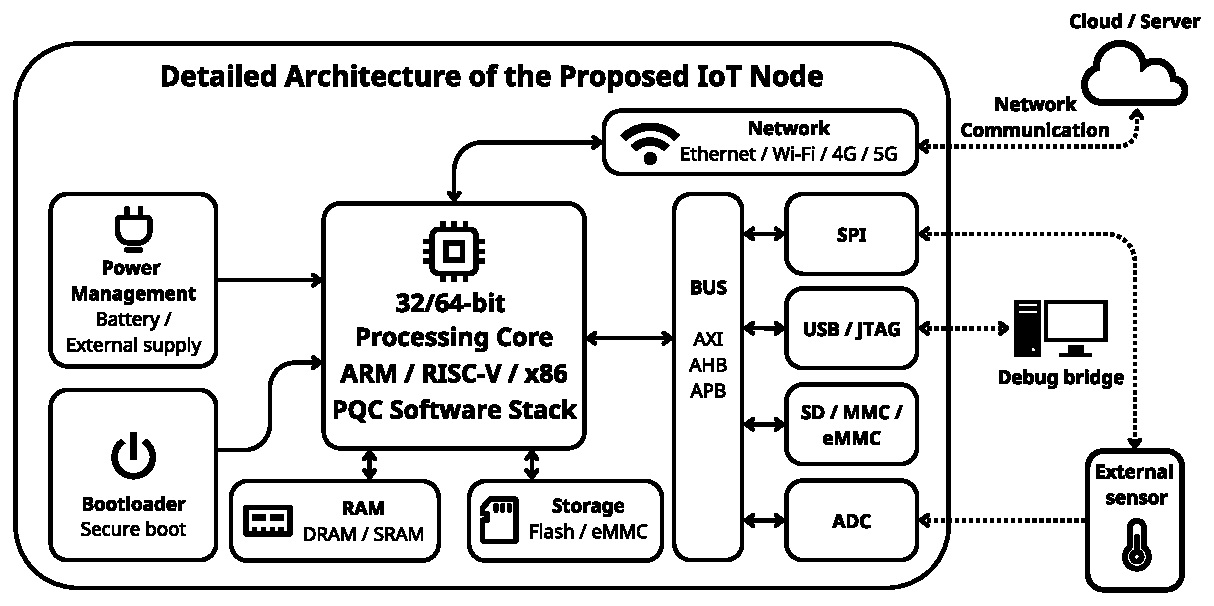
\includegraphics[width=0.90\textwidth]{figures/fig1.pdf}
\caption{End-node architecture for PQC-enabled IoT devices.}
\label{fig:end-node}
\end{figure*}

The communication and peripheral side connects the PQC stack to real IoT workloads. Ethernet, Wi-Fi, 4G, or 5G provides the path to the cloud/server for enrollment, telemetry upload, policy update, and authentication exchange. SPI, USB/JTAG, SD/MMC/eMMC, and ADC interfaces connect secure elements, debugging or provisioning tools, local storage, and external sensors. Because PQC public keys, ciphertexts, and signatures may be much larger than classical objects, these data should be staged in shared buffers and moved through the platform bus and high-throughput interfaces rather than repeatedly copied through narrow command paths. This makes the same node architecture scalable from small microcontroller-class devices to Linux-capable edge nodes.

\subsection{Enrollment, authentication, and key rotation}

The platform separates credential enrollment from runtime authentication. During enrollment, the IoT node creates or receives a PQC-capable credential profile that includes the algorithm identifier, public key, parameter set, credential identifier, key usage, and attestation metadata. For a device-bound credential, the private key remains inside the device or its protected execution boundary. The relying-party server stores only the public credential metadata and the associated policy state, while the gateway may cache policy information for constrained or intermittently connected nodes.

During authentication, the server issues a challenge and policy decision for the current session. The node signs the challenge with ML-DSA for device-bound authentication. In a gateway-assisted profile, the gateway verifies that signature or signs under an explicitly delegated gateway credential; it does not receive the node's private key. SLH-DSA is reserved for firmware, audit, or long-term attestation evidence. ML-KEM is used separately to establish a fresh shared secret, and the derived symmetric key protects the IoT data channel. Thus, ML-KEM handles session-key establishment, whereas ML-DSA or SLH-DSA handles authentication and attestation.

Key rotation is handled at the policy layer. When a parameter set is deprecated or a device class becomes too weak, the server can require re-enrollment with a stronger credential profile. For sleeping nodes, the gateway can buffer policy updates and apply them when the node wakes, reducing battery and radio overhead.

\begin{figure*}[t]
\centering
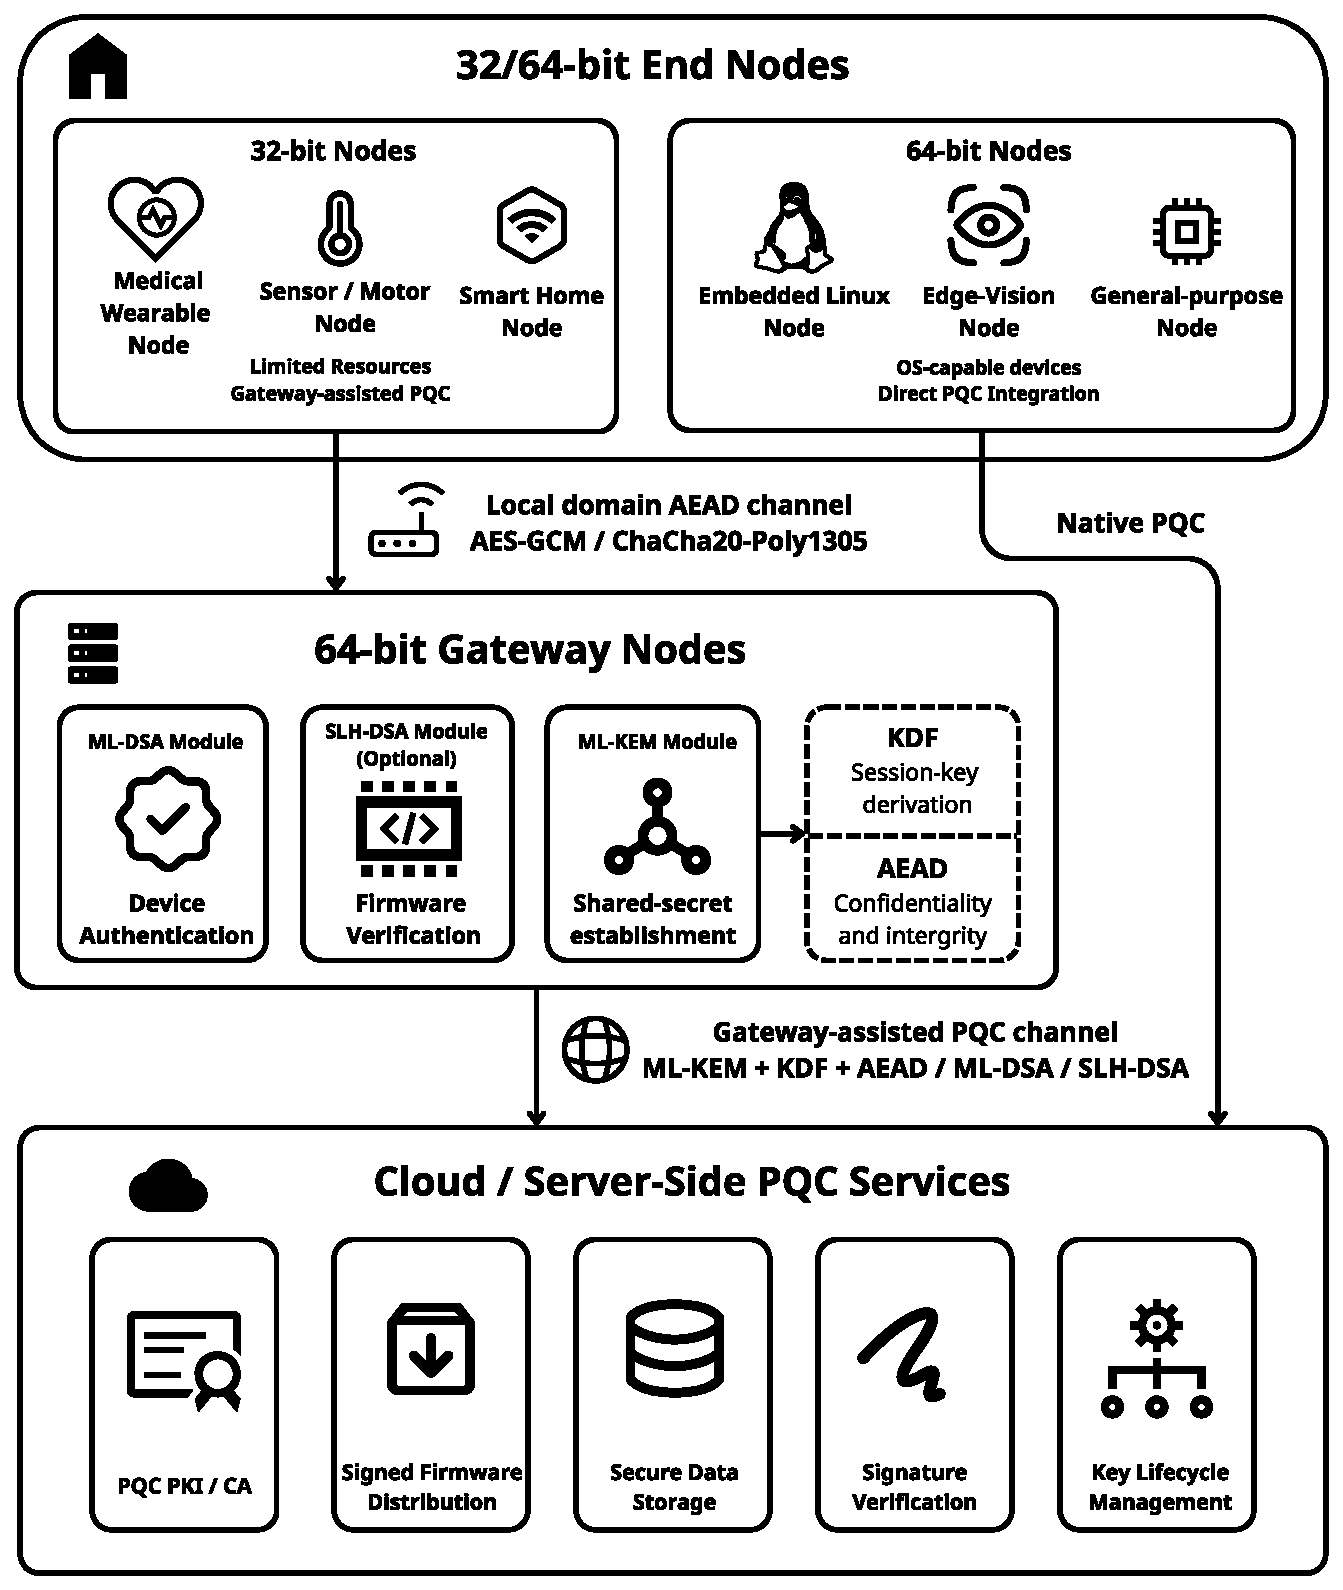
\includegraphics[height=0.62\textheight,keepaspectratio]{figures/fig2.pdf}
\caption{Three-tier deployment map for quantum-safe session establishment and passkey authentication.}
\label{fig:three-tier}
\end{figure*}

Fig.~\ref{fig:three-tier} maps the placement rule to system components. End nodes hold credentials. Capable 64-bit nodes can run direct PQC operations, whereas constrained nodes use the gateway-assisted path. The gateway handles ML-KEM session setup, KDF derivation, AEAD local protection, ML-DSA challenge verification, and optional SLH-DSA firmware or OTA verification. The cloud/server tier provides PQC PKI/CA, signed firmware distribution, secure storage, signature verification, and key lifecycle management. Thus, Table~\ref{tab:placement} becomes an enforceable deployment policy, not just an algorithm list.

\subsection{Security boundaries and failure handling}

The node boundary protects device-bound secrets and performs the minimum cryptographic work needed to authenticate itself. The gateway boundary protects aggregation state, rate limits repeated verification attempts, and prevents a single slow signature operation from blocking all sensor traffic. The server boundary protects long-term policy, audit records, and credential revocation. These boundaries make the system more resilient to partial compromise because a low-end node does not need to hold every policy key or perform every attestation operation.

Failure handling is deliberately conservative. If a node cannot process a required PQC profile, the server can downgrade only to a policy-approved hybrid path and record the event. If a gateway is overloaded, the system can continue accepting telemetry encrypted under a symmetric key established through ML-KEM while delaying noncritical attestation verification. If an SLH-DSA signature is required for firmware or audit records, the platform does not silently replace it with a lighter algorithm; it schedules the operation at a tier that can handle the cost. This prevents performance optimization from weakening the security objective.

\section{Experiment and Results}

\subsection{Experimental setup}

The prototype evaluation used reference-style C implementations of Kyber/ML-KEM, Dilithium/ML-DSA, and SPHINCS+/SLH-DSA. Single-operation experiments were executed on Ubuntu Server images in QEMU-based virtual ARM64 and RISC-V targets. The QEMU configuration used one virtual core and 296~MB RAM, with \texttt{NTESTS}~=~10000 for ML-KEM and ML-DSA and \texttt{NTESTS}~=~1000 for SLH-DSA because the hash-based signature family is significantly slower. Additional stress tests simulated high-load IoT conditions with approximately 50 or more concurrent message-processing threads.

The measured outputs include average key generation time, signing or encapsulation time, verification or decapsulation time, end-to-end operation time in the test harness, public key size, secret key size, signature size, ciphertext size, shared secret size, elapsed response time, CPU user time, CPU system time, and maximum resident memory. These metrics were selected because IoT deployment is constrained not only by cryptographic security but also by latency, memory, and link bandwidth.

The experiments were not designed to choose a universal winner. Instead, they expose which operation dominates each deployment tier. For key establishment, the critical values are ciphertext size, decapsulation time, and shared-secret availability. For signatures, the critical values are signing time, verification time, signature length, and the number of concurrent verification requests that a gateway can absorb. This tier-oriented view is more useful for IoT architecture than a single average runtime number.

The evaluation is tied to three architectural questions. First, it checks whether ML-KEM ciphertext sizes and decapsulation latency are small enough for node-side session establishment. Second, it compares ML-DSA and SLH-DSA as authentication candidates under both single-operation and concurrent workloads. Third, it records resident memory and payload size to determine whether an operation should remain on the node or be moved to the gateway/server tier. The results are therefore used as placement evidence, not as final cycle-accurate hardware characterization.

\subsection{Single-operation observations}

The QEMU results support the proposed placement policy. On the tested ARM64 target, ML-KEM end-to-end operation time was approximately 1.00~ms for Kyber512, 1.40~ms for Kyber768, and 2.02~ms for Kyber1024. ML-DSA was heavier but still practical for measured authentication workflows, with end-to-end values of approximately 4.07~ms for Dilithium2, 6.42~ms for Dilithium3, and 8.41~ms for Dilithium5. On the selected RISC-V configuration, the same operations remained in a similar order of magnitude but were generally slower.

SLH-DSA behaved differently. For selected RISC-V 64-bit SPHINCS+ parameters, sha2-128f-simple signed in about 205.06~ms with a 17088-byte signature, while shake-256f-robust signed in about 2508.36~ms with a 49856-byte signature. These values show that SLH-DSA is not a good default for frequent low-latency IoT messages. The architecture therefore treats SLH-DSA as a gateway/server operation or an infrequent firmware and audit operation.

\begin{table}[t]
\caption{Stress workload summary from the prototype measurement}
\label{tab:stress}
\centering
\scriptsize
\renewcommand{\arraystretch}{1.08}
\setlength{\tabcolsep}{2.5pt}
\begin{tabularx}{\columnwidth}{@{}>{\raggedright\arraybackslash}p{0.20\columnwidth}Y>{\raggedright\arraybackslash}p{0.23\columnwidth}@{}}
\toprule
\textbf{Algorithm} & \textbf{Measured stress metrics (elapsed, RSS, payload)} & \textbf{Recommended tier} \\
\midrule
Dilithium2 & 1110.97~ms, 628~KB, 2420~B sig. & Node/gateway \\
Dilithium3 & 1406.81~ms, 660~KB, 3309~B sig. & Gateway \\
Dilithium5 & 1768.26~ms, 704~KB, 4627~B sig. & Gateway \\
Kyber512 & 1589.82~ms, 704~KB, 768~B ct. & Node \\
Kyber768 & 1584.53~ms, 644~KB, 1088~B ct. & Node \\
Kyber1024 & 1822.05~ms, 652~KB, 1568~B ct. & Node/gateway \\
SPHINCS+ & 29463.60~ms, 612~KB, 17088~B sig. & Server \\
\bottomrule
\end{tabularx}
\end{table}

\subsection{Stress-test analysis}

Table~\ref{tab:stress} summarizes the stress workload. The signature-based algorithms show a direct payload penalty: Dilithium grows from 2420 to 4627 bytes across the tested security levels, while SPHINCS+ reaches 17088 bytes and approximately 29.46~s elapsed time in the measured stress workload. The Kyber family has smaller ciphertexts, from 768 to 1568 bytes. This supports the decision to keep ML-KEM at the node and to avoid per-message SLH-DSA signing at the edge.

The memory column in Table~\ref{tab:stress} is a Linux/QEMU resident-set measurement, not a direct SRAM-footprint estimate for an ESP32-class microcontroller. It should therefore be used as a relative software-side indicator rather than as proof that the same workload fits unchanged in microcontroller SRAM. The dominant constraint is the combination of response time, payload length, and concurrency. A node that transmits small sensor messages over a low-bandwidth link can spend more bandwidth on the signature than on the application data. Therefore, the proposed platform batches, aggregates, or offloads heavy signatures at the gateway. For message-level confidentiality, the node establishes a shared secret using ML-KEM and then encrypts the application stream with a symmetric cipher.

These results should be interpreted as prototype measurements rather than final silicon characterization. QEMU is useful for comparing software flows and parameter sets, but final deployment should include power measurement, real radio throughput, flash-wear analysis, and timing-leakage tests on physical boards. Nevertheless, the relative behavior is sufficient to guide the proposed tiering rule: lattice-based KEM and DSA are practical building blocks for node/gateway workflows, while hash-based signatures are better used at lower frequency or at a higher-resource tier.

\subsection{Design implications}

The first implication is that PQC integration should be buffer-first. Static buffers sized for classical signatures are not enough. Firmware should define separate buffers for KEM ciphertexts, digital signatures, credential metadata, and application payloads, then enforce maximum sizes at compile time. This avoids accidental stack growth and makes memory pressure visible during review. For RTOS-based nodes, long signatures should be allocated in controlled memory regions rather than on small task stacks.

The second implication is that authentication should be rate-aware. A gateway that verifies many signatures concurrently may become the bottleneck even if each individual verification is acceptable. The gateway therefore needs queues, timeouts, and admission control. When traffic bursts occur, telemetry encrypted under a symmetric key established through ML-KEM can continue while noncritical audit signatures are deferred. This is useful in sensor fleets where data freshness and identity assurance have different real-time requirements.

The third implication is that hardware acceleration should target the dominant kernels rather than the protocol wrapper. For lattice-based schemes, polynomial arithmetic and number-theoretic transform units are natural acceleration targets. For hash-based signatures, SHA-2 and SHAKE throughput dominate. In an accelerator-equipped variant, a future FPGA or ASIC implementation should expose memory-mapped accelerator registers and buffer descriptors so that the software stack can reuse the same policy and buffer architecture described in Fig.~\ref{fig:end-node}. This keeps hardware acceleration aligned with the proposed platform model: the node, gateway, or server may accelerate the expensive kernel, but the credential profile, buffer ownership, and placement policy remain controlled by software.

Finally, the implementation should make policy decisions observable and testable. A verifier should be able to determine which credential profile, parameter set, hybrid state, and gateway-offload decision was used for each authentication event. This reduces ambiguity during migration, supports audit and revocation, and prevents an overloaded gateway from silently replacing a required high-assurance operation with a weaker one.

\section{Conclusion}

This paper proposed a scalable Edge-IoT platform for post-quantum authentication and session establishment. The design connects NIST-standardized PQC algorithms with a WebAuthn-style credential model, a hybrid migration policy, and an embedded data path for large PQC objects. The central idea is algorithm placement: ML-KEM is kept close to the node for efficient session-key establishment, ML-DSA supports challenge-response authentication at the node or gateway tier, and SLH-DSA is used selectively for high-assurance but infrequent attestation.

The prototype measurements support this division. ML-KEM and ML-DSA have manageable latency and payload sizes in the measured node/gateway workflow, whereas SLH-DSA provides a conservative hash-based option at the cost of much larger signatures and higher signing latency. The stress-test analysis further shows that payload size and concurrency can dominate the design even when peak resident memory is acceptable. These findings motivate buffer-first firmware design, gateway-side rate control, and hardware acceleration focused on polynomial arithmetic, NTT, SHA-2, and SHAKE kernels.

The current evaluation remains software-centric and simulation-assisted. Future work will implement the architecture on physical ESP32, ARM, and RISC-V boards; measure power, flash wear, radio throughput, and timing leakage; and compare the platform with existing PQC IoT architectures under larger concurrent workloads. This will convert the proposed migration baseline into a board-level implementation suitable for deployment-oriented evaluation.

\bibliographystyle{IEEEtran}
\bibliography{references}

\end{document}
